\documentclass{beamer}
\newcommand{\name}{Kai }
\usetheme{Berlin}
\usecolortheme{beaver}
\usepackage[german]{babel}
\usepackage{graphicx}
\usepackage{xcolor}
\begin{document}
\title{NSD Skills Projekt}
\author{Kai Renken}
\date{\today}

\frame{\titlepage}
\setcounter{tocdepth}{1}

\frame{\frametitle{Ablauf}\tableofcontents}

\section{Was ist das Skills-Projekt?} 
\frame{\frametitle{Überblick}
	\begin{itemize}
		\pause
		\item Wir bauen eine Anwendung zur Organisation der Fähigkeiten (Skills) von Mitarbeitern bei neusta.
		\pause
		\item Es gibt einen Katalog mit verfügbaren Skills inklusive einer Gewichtung. (Relevanz für das Unternehmen)
		\pause
		\item Diese Skills sind Kategorien zugeordnet.
		\pause
		\item Es gibt ein Portal, um meine Skills zu erfassen. \\ (Wie gut kann ich was?)
		\pause
		\item Ich kann Erfolge sammeln. (Stichwort "Gamification")
		\pause
		\item Über meine Skills und Erfolge kann ich einem Profil zugeordnet werden. (Junior, Professional, Senior)
		\pause
		\item Das aktuelle Profil kann Grundlage transparenterer Gehaltsverhandlungen sein. (Stichwort: "Gehaltsbänder")
	\end{itemize}
}

\section{Wie funktioniert das genau?}
\frame{\frametitle{Ich möchte mehr Geld verdienen!}
	\begin{itemize}
		\pause
		\item Ich bin \name und möchte mehr Geld verdienen!
		\pause
		\item Aktuell verdiene ich 48.000 € Jahresgehalt.
		\pause
		\item Meine \textcolor{blue}{Rolle} ist Java-Entwickler.
		\pause
		\item Mein \textcolor{blue}{Profil} ist Junior.
		\pause
		\item Als Junior-Java-Entwickler beginnt mein Gehaltsband bei 42.000 € Jahresgehalt.
		\pause
		\item Es gibt die Profile \textcolor{red}{Junior}, \textcolor{red}{Professional} und \textcolor{red}{Senior}
	\end{itemize}
}

\frame{\frametitle{Wie werde ich Professional?}
	\pause
	Für das Profil Professional-Java-Entwickler gelten folgende Voraussetzungen:
	\begin{itemize}
		\pause
		\item Der Erfolg 'Datenbanken (erweitert)'
		\pause
		\item Der Skill 'IntelliJ IDEA Shortcuts kennen' mit mindestens 5 Punkten
	\end{itemize}
}

\frame{\frametitle{Wie gut beherrsche ich einen Skill?}
	\pause
	Pro Skill kann ich erfassen, für wie kompetent ich mich dabei halte, nämlich:
	\begin{itemize}
		\pause
		\item Ich habe keine Ahnung, habe aber Interesse daran
		\pause
		\item Ich habe Grundlagenkenntnisse
		\begin{itemize}
			\pause
			\item wenig
			\pause
			\item mittel
			\pause
			\item viel
		\end{itemize}
		\pause
		\item Ich habe fundierte Kenntnisse
		\begin{itemize}
			\pause
			\item wenig
			\pause
			\item mittel
			\pause
			\item viel
		\end{itemize}
		\item Ich habe Expertenkenntnisse
		\begin{itemize}
			\pause
			\item wenig
			\pause
			\item mittel
			\pause
			\item viel
		\end{itemize}
	\end{itemize}
}

\frame{\frametitle{Wie werde ich Professional?}
	Für das Profil Professional-Java-Entwickler gelten folgende Voraussetzungen:
	\begin{itemize}
		\item Der Erfolg 'Datenbanken (erweitert)'
		\item Der Skill 'IntelliJ IDEA Shortcuts kennen' mit mindestens 5 Punkten
	\end{itemize}
}

\frame{\frametitle{Wie werde ich Professional?}
	Für den Erfolg 'Datenbanken (erweitert)' gelten folgende Voraussetzungen:
	\begin{itemize}
		\pause
		\item Mindestens 20 Punkte aus der Kategorie 'SQL-Datenbanken'
		\pause
		\item Der Erfolg 'Datenbanken (Grundlagen)'
		\pause
		\item Der Skill 'Hibernate' mit mindestens 2 Sternen
	\end{itemize}
	\pause
	Ich erfülle sonst alle Voraussetzungen, aber kenne mich nicht mit Hibernate aus. \\
	\pause
	Ich nehme mir also etwas Zeit, mich mit Hibernate zu beschäftigen. \\
	\pause
	Jetzt fühle ich mich einigermaßen sicher im Umgang mit Hibernate und trage für den Skill 2 Sterne im Portal ein. \\
	\pause
	Damit bin ich jetzt Professional-Java-Entwickler.
}

\frame{\frametitle{Auf geht's zur Gehaltsverhandlung!}
	\pause
	Das Gehaltsband für das Profil Professional-Java-Entwickler beginnt bei 55.000 €. \\
	\pause
	Da ich aktuell nur 48.000 € verdiene ist mir also eine Gehaltserhöhung von mindestens 7.000 € sicher. \\
}

\frame{\frametitle{Domänenmodell}
	\centering
	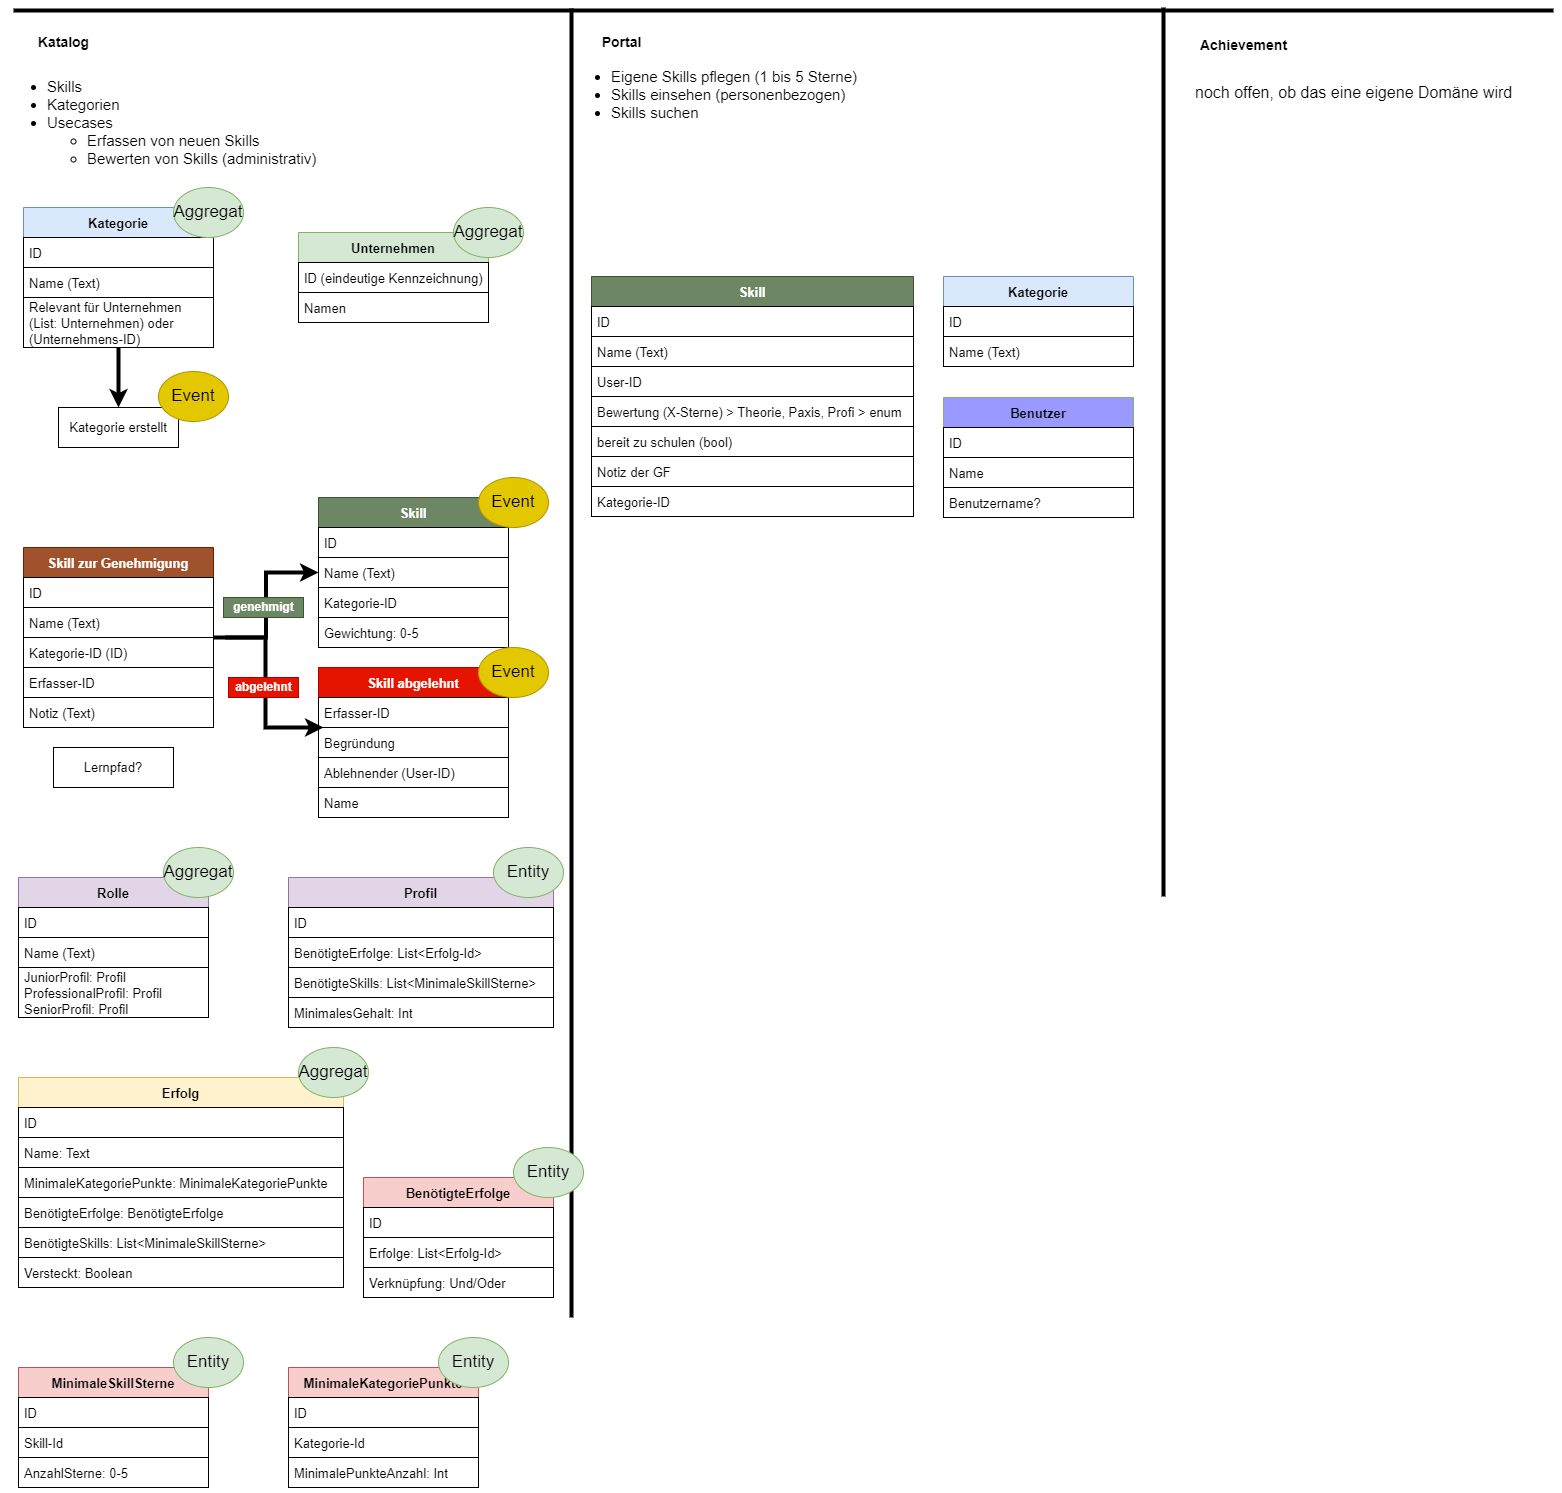
\includegraphics[scale=0.1]{domain_model.png}
}

\section{Technischer Rahmen}

\frame{\frametitle{Architektur / Tech-Stack}
	\begin{itemize}
		\pause
		\item Kotlin
		\pause
		\item Maven
		\pause
		\item Spring Boot
		\pause
		\item PostgreSQL
		\pause
		\item Hexagonale Architektur
		\pause
		\item Domain Driven Design
		\pause
		\item Microsoft Azure AD
		\pause
		\item Kubernetes
	\end{itemize}
}

\section{Werbung}

\frame{\frametitle{Aktueller Stand}
	\centering
	\url{http://nsdskillz-katalog.intern.neusta.de/}
}

\frame{\frametitle{Inner Source}
	Wer mitmachen will, meldet sich einfach bei:
	\begin{itemize}
		\item Lars Michaelis
		\item Lars Mühlmann
		\item Kai Renken
		\item Fabian Wolf
	\end{itemize}
}

\end{document}
